\documentclass[web]{frama-c-book}

\usepackage{graphicx,calc,wrapfig,tikz}

\newcommand{\framacversion}{\input{../../VERSION}}

\newcommand{\tool}[1]{\textsf{#1}\xspace}

\newcommand{\C}{\tool{C}}
\newcommand{\caml}{\tool{OCaml}}
\newcommand{\acsl}{\tool{ACSL}\index{ACSL@\tool{ACSL}}}
\newcommand{\gcc}{\tool{GCC}}
\newcommand{\Value}{\tool{Value}}
\newcommand{\framac}{\tool{Frama-C}}
\newcommand{\stady}{\tool{StaDy}}
\newcommand{\pathcrawler}{\tool{PathCrawler}}

\newenvironment{commands}%
{\par\hspace{2cm}\begin{tabular}{l}}%
{\end{tabular}}

\newcommand{\via}{\emph{via}\xspace}
\newcommand{\etc}{\emph{etc}\xspace}
\newcommand{\ie}{\emph{i.e.}\xspace}
\newcommand{\eg}{\emph{e.g.}\xspace}

% Index

\newcommand{\optionidx}[2]{\index{#2@\texttt{#1#2}}}
\newcommand{\codeidx}[1]{\index{#1@\texttt{#1}}}
\newcommand{\scodeidx}[2]{\index{#1@\texttt{#1}!#2@\texttt{#2}}}
\newcommand{\sscodeidx}[3]{%
  \index{#1@\texttt{#1}!#2@\texttt{#2}!#3@\texttt{#3}}}
\newcommand{\bfit}[1]{\textbf{\textit{\hyperpage{#1}}}}
\newcommand{\optionidxdef}[2]{\index{#2@\texttt{#1#2}|bfit}}
\newcommand{\codeidxdef}[1]{\index{#1@\texttt{#1}|bfit}}
\newcommand{\scodeidxdef}[2]{\index{#1@\texttt{#1}!#2@\texttt{#2}|bfit}}
\newcommand{\sscodeidxdef}[3]{%
  \index{#1@\texttt{#1}!#2@\texttt{#2}!#3@\texttt{#3}|bfit}}

\newcommand{\pragmadef}[1]{\texttt{#1}\index{Pragma!#1@\texttt{#1}}}
\newcommand{\optiondef}[2]{\texttt{#1#2}\optionidxdef{#1}{#2}}
\newcommand{\textttdef}[1]{\texttt{#1}\codeidxdef{#1}}

\newcommand{\optionuse}[2]{\texttt{#1#2}\optionidx{#1}{#2}}
\newcommand{\textttuse}[1]{\texttt{#1}\codeidx{#1}}

% Special environment
\definecolor{gris}{gray}{0.85}

\makeatletter
\newenvironment{important}%
{\hspace{5pt plus \linewidth minus \marginparsep}%
 \begin{lrbox}{\@tempboxa}%
   \begin{minipage}{\linewidth - 2\fboxsep}}
{\end{minipage}\end{lrbox}\colorbox{gris}{\usebox{\@tempboxa}}}
\makeatother

\newtheorem{convention}{Recommendation}[chapter]


\makeindex

\begin{document}

\coverpage{StaDy Manual}

\begin{titlepage}
\begin{flushleft}

\includegraphics[height=14mm]{cealistlogo.jpg}
\end{flushleft}
\vfill
\title{StaDy Manual}{Release \framacversion}
\author{Guillaume Petiot and Nikolay Kosmatov}
\begin{tabular}{l}
CEA LIST, Software Safety and Security Laboratory, Saclay, F-91191 \\
\end{tabular}
\vfill
\begin{flushleft}
  \textcopyright 2015 CEA LIST

This work has been supported by the project STANCE (FP7 317753).
\end{flushleft}
\end{titlepage}

\tableofcontents

%%%%%%%%%%%%%%%%%%%%%%%%%%%%%%%%%%%%%%%%%%%%%%%%%%%%%%%%%%%%%%%%%%%%%%%%%%%%%%%

%% \chapter*{Foreword}
%% \markright{}
%% \addcontentsline{toc}{chapter}{Foreword}

%% This is the user manual of \FramaC\footnote{\url{http://frama-c.com}}.  The
%% content of this document corresponds to the version \framacversion (\today) of
%% \FramaC. However the development of \FramaC is still ongoing: features
%% described here may still evolve in the future.

%% \section*{Acknowledgements}

%% We gratefully thank all the people who contributed to this document: Patrick
%% Baudin, Mickaël Delahaye, Philippe Hermann, Benjamin Monate and Dillon Pariente.

%%%%%%%%%%%%%%%%%%%%%%%%%%%%%%%%%%%%%%%%%%%%%%%%%%%%%%%%%%%%%%%%%%%%%%%%%%%%%%%

\chapter{Introduction}



Among
% the most powerful modern
formal verification techniques, \emph{deductive verification}
% can be used to prove
consists in establishing a rigorous mathematical proof that a given
% annotated
program meets its specification. When no confusion is possible, one also says
% for short
that deductive verification consists in ``proving a program''. It requires that
the program comes with a formal specification, usually given in special comments 
called \emph{annotations,} including function contracts (with
pre- and postconditions) and loop contracts (with loop variants and invariants).
The \emph{weakest precondition calculus} proposed by
Dijkstra~\cite{DBLP:books/ph/Dijkstra76} reduces any deductive verification
problem to %the one of 
establishing the validity of first-order
formulas called \emph{verification conditions}.
% is based on \emph{Weakest-Precondition calculus}
% initiated by Hoare, Floyd and Dijkstra in the late 1960's
%Hoare [Hoa69], Floyd [Flo67] and Dijkstra [Dij68]
% (see e.g. \cite{Hoare1969}) and


In modular deductive verification of a function $f$ calling another function
$g$, the roles of the pre- and postconditions of $f$ and of the callee $g$ are
dual.
% (see Fig.~\ref{fig:VerifFuncCall}).
The precondition of $f$ is assumed and its  postcondition must be proved, while
at  any call of $g$ in $f$, %\commentNK{ambiguous otherwise} 
the precondition of
$g$ must be proved before the call and its postcondition is assumed after the
call.
The situation for a function $f$ with one call to $g$ is presented in
Fig.~\ref{fig:verif-func-call}.
An arrow in this figure informally indicates that its initial point provides a
hypothesis for a proof of its final point.
% in Fig.~\ref{fig:verif-func-call} informally indicate basic implications to be
% proved for a function with one function call.
For instance, the precondition $\textit{Pre}_f$ of $f$ and the postcondition
$\textit{Post}_g$ of $g$ provide hypotheses for a proof of the postcondition
$\textit{Post}_f$ of $f$.
% formalizes this informal presentation).
The called function $g$ is proved separately.


%===========================================================
\input FigVerifFuncCall.tex
%===========================================================

To reflect the fact that some contracts become hypotheses
during deductive verification of $f$
we use the term \emph{subcontracts for $f$} 
to designate contracts of called functions and loops in $f$.


\textbf{Motivation.} 
One of the most important difficulties in deductive verification is the manual
processing of proof failures 
%that must be manually analyzed 
by the verification engineer since proof failures may have several
causes. 
Indeed, a failure to prove $\textit{Pre}_g$ in Fig.~\ref{fig:verif-func-call} may be due to
a \emph{non-compliance} of the code to the specification:
an error in the code \lstinline'code1', or a 
wrong specification $\textit{Pre}_f$ or $\textit{Pre}_g$ itself
that may incorrectly formalize the requirements.
The verification can also remain inconclusive because of 
a \emph{prover incapacity} to finish
a particular proof within an allocated time. 

In many cases, it is extremely difficult for the verification engineer 
to decide how to proceed: 
either suspect a non-compliance and look for an error in the code or check the specification, 
or suspect a prover incapacity, give up automatic proof and try to achieve an
interactive proof with a proof assistant (like \textsc{Coq} \cite{coq}).

A failure to prove the postcondition $\textit{Post}_f$ %in the situation shown in
(cf. Fig.~\ref{fig:verif-func-call}) is even more complex to analyze: along with a
prover incapacity or a non-compliance due to errors in the pieces of code
\lstinline'code1' and \lstinline'code2' or an incorrect
% due to an wrong
specification $\textit{Pre}_f$ or $\textit{Post}_f$, the failure can
also result from a \textit{too weak} postcondition $\textit{Post}_g$ of $g$, that
does not fully express the intended behavior of $g$. Notice that in this last case, the proof of $g$ can
still be successful. 
%However, 
The current automated tools for program proving
do not provide a precise 
% the verification engineer receives
indication on the reason of the proof failure.
%Some of them do not give any reason (like \framac/\Wp).
The most advanced tools (like \tool{Dafny} \cite{Leino/FIDE14}) produce a
counter-example extracted from the underlying solver
that cannot precisely indicate if the verification engineer should look for 
a non-compliance,
or strengthen subcontracts (and which one of them), 
or consider adding additional lemmas or using interactive proof.
So the verification engineer must basically consider all possible reasons one
after another, maybe also trying a very costly interactive proof.
For a loop, %(cf. Fig.~\ref{fig:verif-loop})
the situation is similar,
and offers an additional challenge:
to prove the invariant preservation, whose failure 
can be due to several reasons as well.


The motivation of this work is twofold. First, we want to provide the
verification engineer with a more precise feedback indicating the reason of each
proof failure. Second, we look for a counter-example that either confirms the
non-compliance and demonstrates that the unproven predicate can indeed fail on a
test datum, or confirms a subcontract weakness
% hypothesis (the contract of a called function or a loop invariant)
showing on a test datum which subcontract is insufficient.
%Absence of counter-examples (at least for a reduced program domain)
%can indicate a prover incapacity to finish the unsuccessful proof.

\textbf{Approach and goals.}
%\commentAG{Ne pas mettre ce qu'on a fait (approach)
%et ce qu'on voudrait atteindre (goal) dans le m\^eme paragraphe.} 
%\commentNK{pas d'accord: comment on approche et pour quel objectif 
%peuvent aller ensemble}
The diagnosis of proof failures 
based on a counter-example generated by a prover can be imprecise
since from the prover's point of view,
the code of callees and loops in $f$ is replaced by the corresponding
subcontracts.
To make this diagnosis more precise, one should  
take into account their code as well as their contracts.
A recent study~\cite{Tschannen/14} proposed to use function inlining and loop unrolling.
We propose an alternative approach: to
use advanced test generation techniques in order to diagnose 
proof failures and produce counter-examples.
Their usage requires a translation of the annotated
%\commentAG{Ajouter une phrase
%expliquant la notion d'annotation de sp\'ecification en commentaire dans les
%langages de programmation usuels, ou ne jamais parler d'annotation.} 
%\commentNK{fait}
C program
into an executable C code suitable for testing.
%\commentAG{Cette notion de
%``suitable for testing'' est à mieux définir ou à reformuler.} 
%\commentNK{Not a term here, just English words}
Previous work
% \cite{Petiot/TAP14,Petiot/SCAM14}
addressed the generation of counter-examples by testing only for a
non-compli\-ance \cite{Petiot/TAP14} and proposed a rule-based formalization of
annotation translation
% into C code suitable to produce counter-examples by test generation
in that case~\cite{Petiot/SCAM14}.
The cases of subcontract weakness remained undetected and indistinguishable from
a prover incapacity.

The overall goal of the present work is to provide a methodology for a more
precise  identification of proof failure reasons in all these cases, to
implement it and to evaluate it in practice.
The proposed method is composed of two steps. The first step looks for
non-compliance. If no non-compliance is detected, the second step looks for a
subcontract weakness.
%\commentNK{Subcontract or Contract?} 
Another goal is to make this method automatic and suitable for a non-expert verification
engineer.
Following the modular verification approach,
we assume that the called functions have been verified before the caller $f$.
%, and the called functions respect their contracts.
To simplify the presentation, we also assume that 
the loops preserve their loop invariants, and focus
on other proof failures occurring during modular verification of $f$. 
(The proposed techniques can be adapted to the verification of a loop contract.)

%%%%%%%%%%%%%%%%%%%%%%%%%%%%%%%%%%%%%%%%%%%%%%%%%%%%%%%%%%%%%%%%%%%%%%%%%%%%%%%

\chapter{Installation}


\stady requires \framac Sodium (20150201) and \pathcrawler Sodium. It also requires the GMP (Gnu Multi-Precision) library to be installed.

You can check the version of \framac with :

\begin{shell}
  frama-c -version
\end{shell}

You can compile \stady from the sources this way :

\begin{shell}
  autoconf
  ./configure
  make
  make install
\end{shell}


%%%%%%%%%%%%%%%%%%%%%%%%%%%%%%%%%%%%%%%%%%%%%%%%%%%%%%%%%%%%%%%%%%%%%%%%%%%%%%%

\chapter{Functioning and user interface}

The \stady prototype has two main functionalities : non-compliance detection and subcontract weakness detection.

\section{Non-compliance detection}

\stady tries to exhibit a test case whose execution provokes an annotation violation. Non-compliance detection is the default mode of \stady. One can detect non-compliances between the code and its specification in file $F$, starting with function $M$, using the command :

\begin{shell}
frama-c F -main M -stady
\end{shell}

In the user interface of \framac, an annotation violation is pictured with a red bullet, as we can see in Fig.~\ref{fig:gui}.

\begin{figure}\centering
  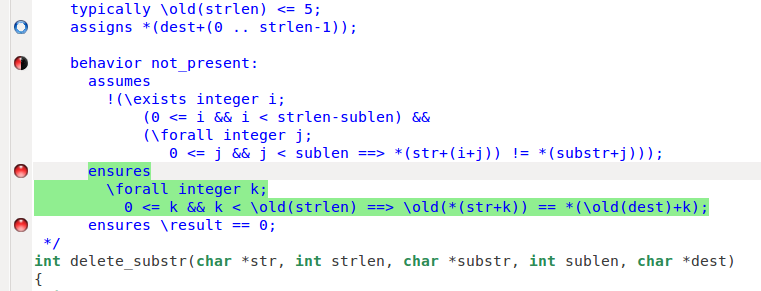
\includegraphics[scale=.4]{ppt_invalid.png}
  \caption{Invalid annotation in the Graphical User Interface of \framac
    \label{fig:gui}}
\end{figure}

\section{Subcontract weakness detection}

\stady tries to exhibit a test case whose execution does not provoke an annotation violation but that is not proved by deductive verification because of a too weak subcontract (loop invariant or called function contract). The subcontract weakness detection in file $F$ starting with function $M$ is done with :

\begin{shell}
  frama-c F -main M -stady -stady-swd C
\end{shell}

where C is a comma-separated list of subcontract identifiers. The subcontract identifiers are the statement identifiers of the corresponding loops (for loop contracts) and function calls (for function contracts).

For now, there is no strategy or heuristic implemented in \stady to automatically submit a set of subcontract identifiers.

%%%%%%%%%%%%%%%%%%%%%%%%%%%%%%%%%%%%%%%%%%%%%%%%%%%%%%%%%%%%%%%%%%%%%%%%%%%%%%%

\chapter{Implementation}


\begin{wrapfigure}[15]{r}{43mm}\centering
  \tikzstyle{data}=[node distance=1.4cm]
  \tikzstyle{action}=[draw,rectangle,node distance=1.4cm]
  \tikzstyle{expl}=[text width=6cm,node distance=6cm,align=left]
  \begin{tikzpicture}[>=latex,font=\scriptsize]
    \node[data] (annot-p) {Annotated C program};
    \node[action,below of=annot-p] (transl) {\textbf{(1)} Translation};
    \node[data,below of=transl] (instr-p) {Instrumented C program};
    \node[action,below of=instr-p] (test-gen){\textbf{(2)} Test generation};
    \node[data,below of=test-gen,align=center] (report) {Counterexamples};
    \draw[->] (annot-p) -- (transl);
    \draw[->] (transl) -- (instr-p);
    \draw[->] (instr-p) -- (test-gen);
    \draw[->] (test-gen) -- (report);
  \end{tikzpicture}
  \caption{The two steps of \stady\label{fig:stady-steps}}
\end{wrapfigure}

\stady is composed of two steps :
\begin{itemize}
\item a \textbf{translation} step, producing an instrumented C program from an annotated C program. The ACSL annotations of the latter are translated in a semantically equivalent C code, such that test generation can be applied;

\item a \textbf{test generation} step, trying to cover all feasible execution paths of the program, exhibiting counter-examples if any, and reporting annotation violations. This step uses the \pathcrawler plug-in of \framac.
\end{itemize}

\stady is implemented in OCaml (roughly 3k lines of code). A simplified dependence graph of its modules is presented in Fig.~\ref{fig:stady-deps}.

\begin{figure}\centering
  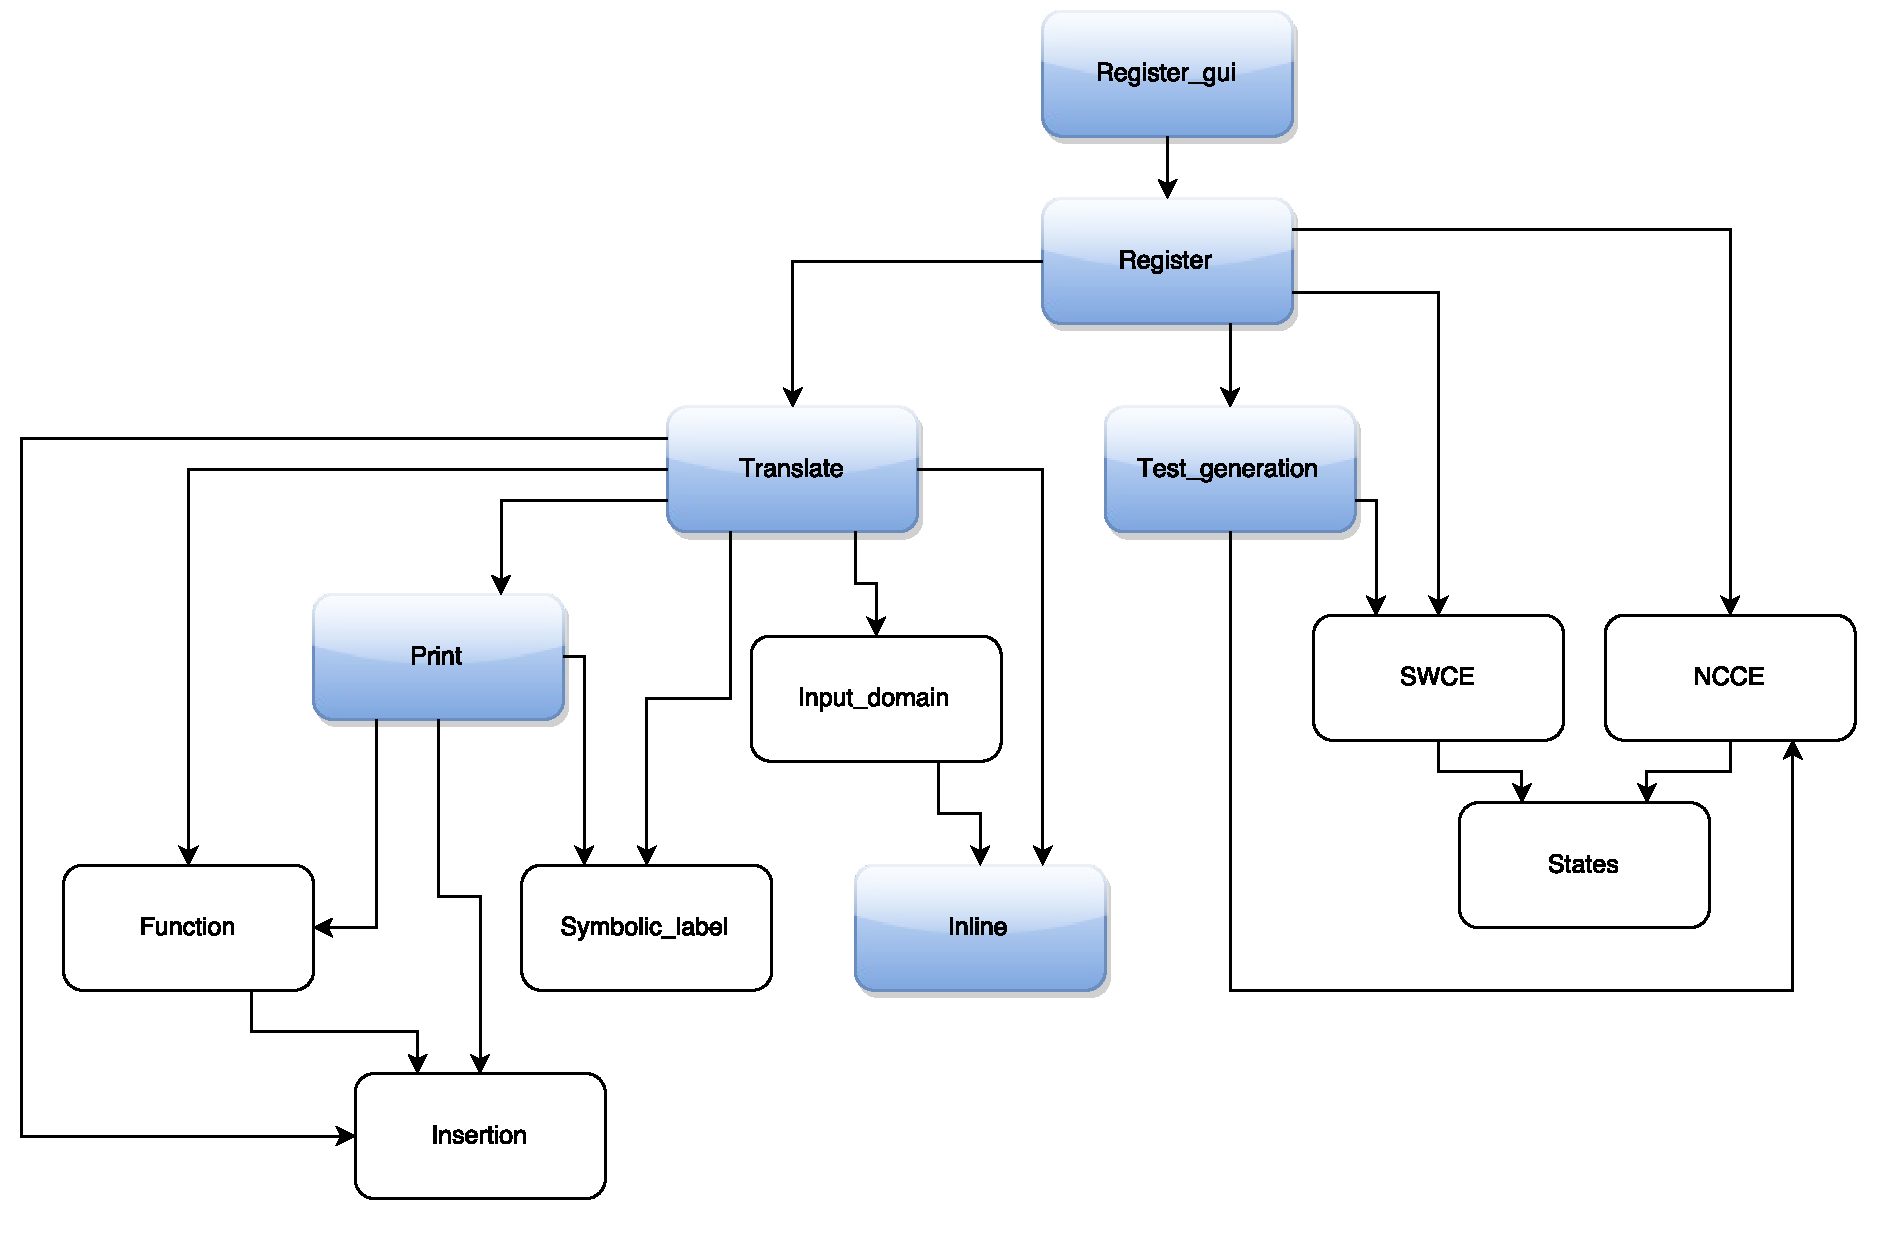
\includegraphics[scale=.5]{stady_architecture.pdf}
  \caption{Dependence graph of \stady\label{fig:stady-deps}}
\end{figure}

Each block of the figure depicts a module or a file, and the relation $A \rightarrow B$ means that $A$ calls $B$. The white blocks correspond to modules describing data types and operations over those types. The coloured blocks correspond to modules implementing an important step or feature of \stady.

The \lstinline[language=OCaml]'Register' module is managing the other modules, whereas \lstinline[language=OCaml]'Register_gui' implements the behaviours of \stady in the Graphical User Interface (GUI) of \framac. The two main features of \stady are : the translation of E-ACSL annotations, performed by the Translate module, and the structural test generation, managed by the \lstinline[language=OCaml]'Test_generation' module. We now present the different operations and modules.

\section{Annotation translation}

In order to translate E-ACSL annotations into C, we need to define specific data types. The \lstinline[language=OCaml]'Insertion' module defines the ``code fragment'' data type. The \lstinline[language=OCaml]'Symbolic_label' module defines symbolic labels that allows the translation to associate a program point to code fragments. Such labels are : beginning or end of a function body, beginning or end of a loop body, before or after a statement. The Function module defines the data type of generated functions. The \lstinline[language=OCaml]'Input_domain' defines the data types encoding the domains and constraints over the program inputs, i.e. the formal parameters of the function that is the entry point of the analysis and the global variables.

The data types defined by the Function and Insertion modules extend the types of the abstract syntax tree (AST) provided by \framac. They allow us not to modify the AST, such as the code fragments are stored outside the AST. Indeed, modifying the AST with \framac plug-ins is very complex because the relations between the data before and after the modification have to be maintained, and this is error-prone. Not modifying the AST allowed us to reduce the development time of \stady.

The \lstinline[language=OCaml]'Inline' module defines a program transformation inlining the logic predicates and logic functions in E-ACSL annotations. In other words, this transformation replaces a call to a predicate or function by its definition and replaces the formal parameters by the effective parameters at call site. This module allows to  handle very easily the annotations involving calls to user-defined predicates or functions, but it does not allow to handle recursive function calls or inductive predicates. The Inline module provides the function pred that inlines a given predicate :

\begin{ocamlcode}
  val pred: Cil_types.predicate -> Cil_types.predicate
\end{ocamlcode}

The \lstinline[language=OCaml]'Translate' module defines the program transformations for the translation of E-ACSL annotations. This module provides a function \lstinline[language=OCaml]'translate' :

\begin{ocamlcode}
  val translate:
    Property.t list -> int list -> precond_fname:string -> instru_fname:string
    -> Property.t list
\end{ocamlcode}

The function \lstinline[language=OCaml]'translate' produces the C file (tagged \lstinline[language=OCaml]'instru_fname') containing the instrumented program and the Prolog file (tagged \lstinline[language=OCaml]'precond_fname') containing the precondition of the function under verification in a format that \pathcrawler can process efficiently. This function returns the list of program properties that have been translated, so that we do not validate non-translated properties by accident. The translation is implemented using an ``in-place visitor'' (opposed to a ``copy visitor'') of \framac. This choice is not disadvantageous because we do not modify the AST and the generated code fragments are stored out of the AST.

The \lstinline[language=OCaml]'Print' module is invoked by the \lstinline[language=OCaml]'Translate' module to write in the output files the result of the translation : the generated functions and the code fragments, inserted at the corresponding labels. This module provides the class \lstinline[language=OCaml]'print_insertions' :

\begin{ocamlcode}
  class print_insertions:
    (Symbolic_label.t, Insertion.t Queue.t) Hashtbl.t -> Function.t list -> int list
    -> Printer.extensible_printer
\end{ocamlcode}

This class is parametrized with the labeled code fragments, the generated functions, the identifiers of subcontracts for Subcontract Weakness Detection (SWD). It defines an object of type \lstinline[language=OCaml]'Printer.extensible_printer' that will be used by the function \lstinline[language=OCaml]'translate' to print the instrumented program in the output files. Once the files are generated, the test generation begins.

\section{Test generation}

We now define the data types we use to handle the test generation results.
The \lstinline[language=OCaml]'NCCE' module implements the data type for Non-Compliance Counter-Examples and functions over this data type : register, retrieve one or many NCCE for a given property. Similarly, the \lstinline[language=OCaml]'SWCE' module implements the data type for Subcontract Weakness Counter-Examples and functions over this data type : register, retrieve one or many SWCE for a given property.

The \lstinline[language=OCaml]'States' module defines the internal states of \stady, such that hash tables storing the NCCE and SWCE generated with \pathcrawler.

The \lstinline[language=OCaml]'Test_generation' module defines an exchange protocol to communicate with \pathcrawler, and opens a socket between \stady and \pathcrawler in order to retrieve the test generation results. This module provides the function \lstinline[language=OCaml]'run' :

\begin{ocamlcode}
  val run:
    entry_point:string -> precondition_filename:string -> instrumented_filename:string
    -> unit
\end{ocamlcode}

The function \lstinline[language=OCaml]'run' constructs the command line to invoke \pathcrawler with the right options, starts the communication with \pathcrawler, registers the test generation results in the \lstinline[language=OCaml]'States', then returns to the \lstinline[language=OCaml]'Register' module at the end of the communication.
\lstinline[language=OCaml]'Register' then updates the properties' status according to the results of test generation.

%%%%%%%%%%%%%%%%%%%%%%%%%%%%%%%%%%%%%%%%%%%%%%%%%%%%%%%%%%%%%%%%%%%%%%%%%%%%%%%

\chapter{Examples}


\section{Non-Compliance Detection}

Let us consider a small example of an array access :

\begin{ccode}
/*@ requires \valid(buffer+(0..size-1)); */
int f(int* buffer, int size, int ind) {
  return buffer[ind];
}
\end{ccode}

The function $f$ takes a buffer, its size, and an index. The precondition on the first line states that we can read and write in \lstinline'buffer[0]', ..., \lstinline'buffer[size-1]'.

First, we apply the \tool{RTE} plug-in of \framac. \tool{RTE} adds an ACSL annotation just before the array access :

\begin{ccode}
  /*@ assert rte: mem_access: \valid_read(buffer+ind); */
\end{ccode}

meaning that buffer has to be large enough so that \lstinline'buffer[ind]' can be read.

\stady is then applied. The full command with the call to \tool{RTE} is :

\begin{shell}
  frama-c buffer.c -main f -rte -then -stady -stady-stop-when-assert-violated
\end{shell}

The option \lstinline[language=shell]'-stady-stop-when-assert-violated' stops the test generation as soon as an annotation violation is detected.
The assertion added by \tool{RTE} is reported as non-compliant with the code, here the output of \stady :

\begin{shell}
[stady] all-paths: true
[stady] 2 test cases
[stady] Non-Compliance of assert rte: mem_access: \valid_read(buffer+ind); 
        LOCATION: buffer.c:4
        TEST DRIVER: testcases___sd_instru_buffer_f/f/testdrivers/TC_1.c
        ind = -214739
        size = 0
\end{shell}

This means that for any buffer of size 0, trying to read the buffer at size 0, will lead to a runtime error.

One can precise the precondition of f to get more meaningful results, we add the following annotations :

\begin{ccode}
  requires 0 <= ind;
  requires 0 < size;
\end{ccode}

Applying \stady again stills exhibits a counter-example :

\begin{shell}
[stady] all-paths: true
[stady] 4 test cases
[stady] Non-Compliance of assert rte: mem_access: \valid_read(buffer+ind); 
        LOCATION: buffer.c:7
        TEST DRIVER: testcases___sd_instru_buffer_f/f/testdrivers/TC_1.c
        buffer[0] = -214739
        ind = 1073652710
        size = 1
\end{shell}

This means that we cannot access \lstinline'buffer[1073652710]' for a buffer of size 1.

We finally correct the precondition :

\begin{ccode}
  requires 0 <= ind < size;
\end{ccode}

This time, there are no more error, so we won't stop at the first annotation violation and we will try each size of buffer (as each size follows its own program path). Thus, we add a timeout to limit the exploration :

\begin{shell}
  frama-c buffer.c -main f -rte -then -stady -stady-stop-when-assert-violated
  -stady-timeout 7
\end{shell}

The option \lstinline[language=shell]'-stady-timeout' limits the time allocated to test generation, here it cannot take more than 7 seconds.
And \stady does not report any annotation violation :

\begin{shell}
[stady] all-paths: true
[stady] 1177 test cases
\end{shell}

\section{Subcontract Weakness Detection}

Let us now consider a more complex program. The function \lstinline'all_zeros' below returns a non-zero value if and only if, all the elements of the array $t$ of size $n$ are non-zero.

\begin{ccode}
/*@ requires n>=0 && \valid(t+(0..n-1));
    assigns \nothing;
    ensures \result != 0 <==> 
      (\forall integer j; 0 <= j < n ==> t[j] == 0);
*/
int all_zeros(int t[], int n) {
  int k;
  /*@ loop invariant 0 <= k <= n;
      loop assigns k;
      loop variant n-k; 
  */
  for(k = 0; k < n; k++) 
    if (t[k] != 0) 
      return 0;
  return 1;
}
\end{ccode}

The deductive verification of the program by the \tool{Wp} plug-in of \framac does not succeed : the postcondition of the function \lstinline'all_zeros' is not verified.

\begin{shell}
[wp] Running WP plugin...
[wp] Collecting axiomatic usage
[wp] warning: Missing RTE guards
[wp] 10 goals scheduled
[wp] [Qed] Goal typed_all_zeros_loop_inv_established : Valid
[wp] [Qed] Goal typed_all_zeros_loop_assign : Valid
[wp] [Qed] Goal typed_all_zeros_assign_part1 : Valid
[wp] [Qed] Goal typed_all_zeros_assign_part2 : Valid
[wp] [Qed] Goal typed_all_zeros_assign_part3 : Valid (1ms)
[wp] [Qed] Goal typed_all_zeros_assign_part4 : Valid (1ms)
[wp] [Qed] Goal typed_all_zeros_loop_term_decrease : Valid (1ms)
[wp] [Qed] Goal typed_all_zeros_loop_term_positive : Valid (1ms)
[wp] [Alt-Ergo] Goal typed_all_zeros_loop_inv_preserved : Valid (Qed:1ms) (44ms) (17)
[wp] [Alt-Ergo] Goal typed_all_zeros_post : Unknown (Qed:2ms) (507ms)
[wp] Proved goals:    9 / 10
     Qed:             8  (0ms-1ms)
     Alt-Ergo:        1  (44ms-44ms) (17) (unknown: 1)
\end{shell}

We can apply \stady to look for a non-compliance between the code and its specification.

\begin{shell}
  frama-c all_zeros.c -main all_zeros -stady -stady-stop-when-assert-violated
  -stady-timeout 5
\end{shell}

\begin{shell}
[stady] all-paths: true
[stady] 19246 test cases
\end{shell}

\stady did not exhibit any counter-example of non-compliance. An enlightened user may get the feeling that the program is correct but insufficiently specified.
We re-apply \stady to look for counter-examples exhibiting subcontract weaknesses :

\begin{shell}
  frama-c all_zeros.c -main all_zeros -stady -stady-swd 2
  -stady-stop-when-assert-violated
\end{shell}

Here, 2 is the identifier of the loop and its contract, it is retrieved by using the GUI of \framac :

\begin{shell}
  frama-c-gui all_zeros.c
\end{shell}

and clicking on the beginning of the while loop, \texttt{statement: 2} is displayed in the Information tab of the GUI. There is no other way to designate a contract for the Subcontract Weakness Detection mode of \stady at the moment.

\begin{shell}
[stady] all-paths: true
[stady] 57 test cases
[stady] Subcontract Weakness of stmt 2 for ensures
                                           \result != 0 <==>
                                           (\forall integer j;
                                              0 <= j < \old(n) ==> *(\old(t)+j) == 0) 
        LOCATION: all_zeros_unproved_1.c:12
        TEST DRIVER: testcases___[...]/all_zeros/testdrivers/TC_9.c
        n = 1
        nondet_sint_val[0] = 1
        return value =  -- OUTPUT: 1 (1)
        t[0] = 6432
\end{shell}

This output means that the loop contract (stmt 2) is not strong enough for the postcondition of the function.
The counter-example has to be read as follows :
\begin{itemize}
\item we consider as inputs : \lstinline'n = 1', \lstinline't[0] = 6432'
\item we replace the execution of the loop by the most general code satisfying its loop contract, that is :
  \begin{itemize}
  \item only $k$ can be modified
  \item the new value of $k$ has to satisfy : \lstinline'0 <= k <= n'
  \end{itemize}
\item a non-deterministic value is thus assigned to $k$ : \lstinline'k = 1' (designated by \lstinline'nondet_sint_val[0]' in the feedback of StaDy)
\end{itemize}
However, this new code for the loop does not change the return value of the function to 0 when one of the element is non-zero, so the new function always returns 1 (OUTPUT: 1 in the feedback of StaDy).

We now realize that we might need a loop invariant over the values of the array elements. We add such a loop invariant (highlighted in yellow) :

\begin{ccode}
/*@ requires n>=0 && \valid(t+(0..n-1));
    assigns \nothing;
    ensures \result != 0 <==> 
      (\forall integer j; 0 <= j < n ==> t[j] == 0);
*/
int all_zeros(int t[], int n) {
  int k;
  /*@ loop invariant 0 <= k <= n;
      loop invariant \forall integer j; 0<=j<k ==> t[j]==0;
      loop assigns k;
      loop variant n-k; 
  */
  for(k = 0; k < n; k++) 
    if (t[k] != 0) 
      return 0;
  return 1;
}
\end{ccode}

With this new loop invariant, \stady does not exhibit any counter-example of contract weakness :

\begin{shell}
  frama-c all_zeros.c -main all_zeros -stady -stady-swd 2 -stady-timeout 5
  -stady-stop-when-assert-violated
\end{shell}

\begin{shell}
[stady] all-paths: true
[stady] 30002 test cases
\end{shell}

And the program can now be formally verified with \tool{Wp} :

\begin{shell}
[wp] Running WP plugin...
[wp] Collecting axiomatic usage
[wp] warning: Missing RTE guards
[wp] 12 goals scheduled
[wp] [Qed] Goal typed_all_zeros_loop_inv_established : Valid
[wp] [Qed] Goal typed_all_zeros_loop_inv_2_established : Valid
[wp] [Qed] Goal typed_all_zeros_loop_assign : Valid
[wp] [Alt-Ergo] Goal typed_all_zeros_loop_inv_2_preserved : Valid (Qed:1ms) (23ms) (24)
[wp] [Alt-Ergo] Goal typed_all_zeros_loop_inv_preserved : Valid (Qed:1ms) (29ms) (17)
[wp] [Alt-Ergo] Goal typed_all_zeros_post : Valid (Qed:3ms) (37ms) (54)
[wp] [Qed] Goal typed_all_zeros_assign_part1 : Valid
[wp] [Qed] Goal typed_all_zeros_assign_part2 : Valid
[wp] [Qed] Goal typed_all_zeros_assign_part3 : Valid (1ms)
[wp] [Qed] Goal typed_all_zeros_assign_part4 : Valid
[wp] [Qed] Goal typed_all_zeros_loop_term_decrease : Valid (1ms)
[wp] [Qed] Goal typed_all_zeros_loop_term_positive : Valid (1ms)
[wp] Proved goals:   12 / 12
     Qed:             9  (0ms-3ms)
     Alt-Ergo:        3  (23ms-37ms) (54)
\end{shell}


%%%%%%%%%%%%%%%%%%%%%%%%%%%%%%%%%%%%%%%%%%%%%%%%%%%%%%%%%%%%%%%%%%%%%%%%%%%%%%%


\appendix


%%%%%%%%%%%%%%%%%%%%%%%%%%%%%%%%%%%%%%%%%%%%%%%%%%%%%%%%%%%%%%%%%%%%%%%%%%%%%%%

\cleardoublepage
\phantomsection
\addcontentsline{toc}{chapter}{\bibname}
\bibliographystyle{plain}
\bibliography{./manual}

%%%%%%%%%%%%%%%%%%%%%%%%%%%%%%%%%%%%%%%%%%%%%%%%%%%%%%%%%%%%%%%%%%%%%%%%%%%%%%%

\cleardoublepage
\phantomsection
\addcontentsline{toc}{chapter}{\listfigurename}
\listoffigures

%%%%%%%%%%%%%%%%%%%%%%%%%%%%%%%%%%%%%%%%%%%%%%%%%%%%%%%%%%%%%%%%%%%%%%%%%%%%%%%

\cleardoublepage
\phantomsection
\addcontentsline{toc}{chapter}{\indexname}
\printindex

\end{document}
